\documentclass{article}
\usepackage{amsmath}
\usepackage{float}
\usepackage{graphicx}
\usepackage{geometry}
\usepackage{tabularx}
\begin{document}
\title{Interferometry}
\author{Xin Gao}
\date{}
\maketitle

\section{Abstract}
Using 1-D, 2-array interferometry, we calculate the baseline length of
our inferometer and the size of the source objects in the sky. Our
sources are the Sun, the Moon, and a point source, the Orion Nebula. In
our analysis of the Orion Nebula, we use a least-squares fitting method
to calculate the baseline length of the interferometer to be 9.925,
slightly off from the approximate but used value of 10. We then
similarly used it along with fringe response equations to derive the
size of the Sun and the Moon in the sky. Their resulting angular values
are close to one another as expected; otherwise, there would be no total
solar eclipses. 
\section{Introduction} 
Interferometry is a core method in radio astronomy for collecting and
analyzing data. An interferometer consists of at least two dish telescopes
that capture signals in radio frequencies. The distance of separation,
or the baseline, is crucial in its design; the precise length determines
the phase difference, if any, of a source signal, which can be used to
extract the declination of the source. It determines the time difference,
or geometric delay, between the reception of the signal by the
telescopes. This delay is used with multiple signals in the method of 
correlation to image the sources. The baseline determines also the phase
difference with a  corresponding wavelength or frequency. This
difference can graphically respresent the signals, manifesting as
sinusoidal 'fringe patterns.' Our analyses use these fringe patterns,
along with statistical and mathematical tools, to derive characteristics
of sources such as their celestial declination, their corresponding
brightness distributions, and, in the case of nearby physically
distinguishable objects such as the Sun and the Moon, their diameter. 

\section{Background: Astrophysics and Conventions for Interferometry}
When studying space, astronomers have to determine a point of reference
for assigning coordinates to objects. There are several conventional
coordinate systems, based on difference reference frames. Similarly,
time conventions exist for determining locations of objects at a
particular time. How astronomers measure light data is also important
for having defined conventions for consistency and communication.
\subsection{Time Conventions for Astronomers}
From the definition of the day to the beginning of dates, astronomers
tend to mess with time for practical purposes.
\subsubsection{The Legacy of Julius}
The dominant dating system being used today is the Gregorian
calendar. In astronomy, Julian dates are used instead. The Julian date
began at noon of present-day England on January 1st, 4713 B.C. and is
counted in solar days. This convention serves as an universal dating
method for astronomers, eliminating confusion due to using different
systems. The Julian Date operates in 7980 year cycles, a value carefully
chosen for convenience and for converting among other dating systems. 
\subsubsection{Solar Days vs. Sidereal Days}
We use the solar day system for our daily lives; that is, we judge the
time of the day by the location of the sun in the sky. Because that
Earth slightly moves its location relative to the sun every day, a solar
day exceeds 2$\pi$ radians about the rotation of the Earth on it axis. A 
sidereal day describes the amount of time that it takes Earth to rotate 
exactly 360 degrees, which results in it lasting approximately 23 hours
and 56 minutes. This convention in the form of Local Sidereal Time (LST)
is useful for calculating the hour angle; this will be explored further.
\begin{figure}[!h]
\centering
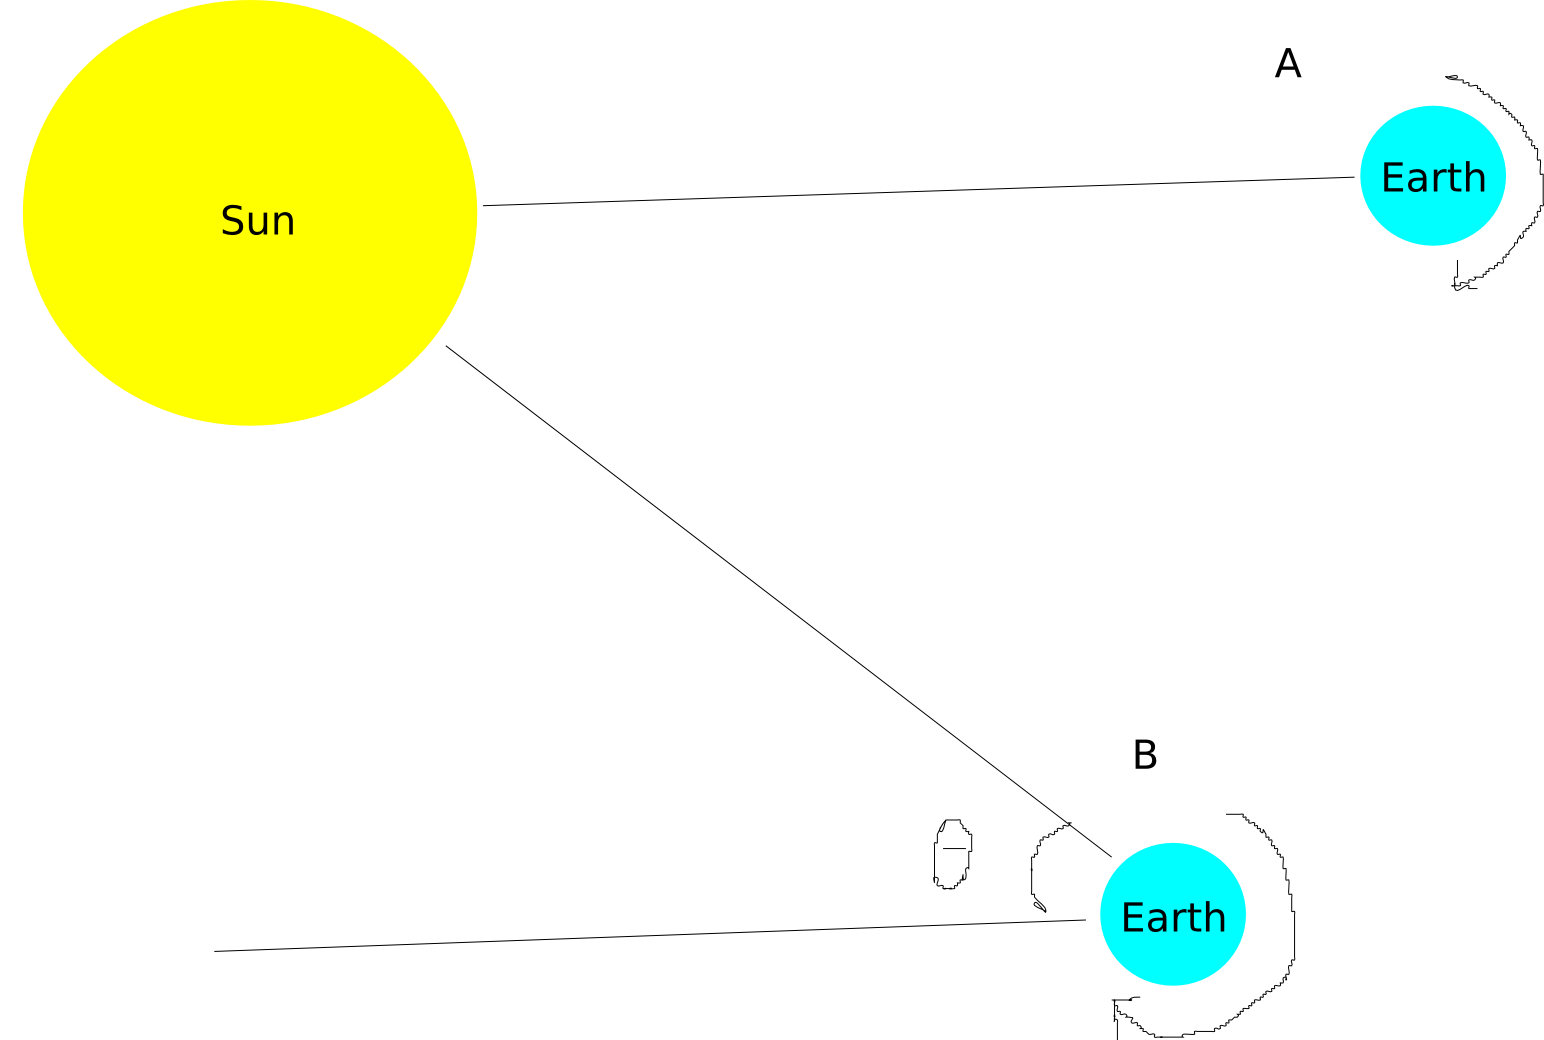
\includegraphics[width=.65\textwidth]{sidereal.png}
\caption{Solar Day vs. Sidereal Day. From point A to point B, the Earth
  made an angle $\theta$ relative to its orbit around the Sun. The
  difference in time of day -for example, the meaning of 'noon'- is also 
described by $\theta$ relative to Earth's rotation about its axis.}
\end{figure}
\subsection{Celestial Reference Frames: Coordinate Systems}
How should we describe the location of an object in the sky? There are
many answers with several conventions to choose from. For our purposes,
the topocentric, hour angle, and equatorial coordinates are of
interest. If one sees a star directly overhead, you might be inclined to 
assign that star an altitude of 90 degrees (zenith). This is in the
reference frame of an individual and the coordinates of an object are
known as to be in topocentric coordinates, measuring an object's azimuth
and altitude \textbf{(az, alt)}. Azimuth value begins at the north
direction and goes counterclockwise. This is convenient for an
individual, but lacks meaning for global communication. For distant
objects, they are in a somewhat fixed position in the sky over long
periods of human time. The equatorial coordinate system, in the
reference frame of the Earth, assigns a fixed coordinate to each
celestial object with a right ascension and declination value 
\textbf{(r$\boldsymbol\alpha, \boldsymbol\delta$)} based on its position
on the celestial sphere. An object in the direction of the sun at vernal
equinox has a right ascension value, measured in hours from 0 to 24, of
0. Increasing values of right ascenion goes with the the path of the sun 
along the elliptic. An object along the celestial equator has a
declination of 0 degrees. 
\begin{figure}[!h]
\centering
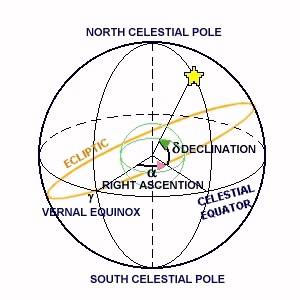
\includegraphics[width=.5\textwidth]{coordinates_equatorial.png}
\caption{Geocentric Equatorial Coordinates with the solar direction on
  spring equinox at the equator, $\gamma$, being the origin.}
\end{figure}
The LST is the current time at a location based on sidereal days. The
hour angle of an object is its right ascension subtracted by the
LST. The hour angle coordinate \textbf{(ha, $\boldsymbol\delta$)} 
describes the right ascension of an object based on an individual's
reference frame but maintains the fixed declination value. We often use
equatorial coordinates and topocentric coordinates with hour angles
coordinates serving as an intermediate system. One set of coordinate
values can be mathematically transformed to that of another by rotation
matrices. The matrix to go from equatorial to hour angle is:
\begin{align}R_{{r\alpha, \delta}\rightarrow{ha, \delta}}
  = \begin{bmatrix}cos(LST) & sin(LST) & 0\\sin(LST) & -cos(LST) & 0\\0
    & 0 & 1\end{bmatrix}
\end{align}
and the matrix to go from hour angle to topocentric is:
\begin{align}R_{{ha, \delta}\rightarrow{az, alt}}
  = \begin{bmatrix}-sin(\phi) & 0 & cos(\phi)\\0 & -1 & 0\\cos(\phi) & 0
    & sin(\phi)\end{bmatrix}
\end{align}
where $\phi$ is latitude of a location in degrees. To go straight from
equatorial to topocentric coordinates, multiply these two matrices of
transformation together in the opposite order. The inverse of this
resulting matrix can be used to go back to equatorial from topocentric
coordinates. We make a python program (in the file rotation\_matrix.py)
to convert coordinates when necessary. Using the sys module, we input
topocentric coordinates for equatorial coordinates as output.
\subsubsection{Perception of Light; Units of Radiation}
There are many ways to categorize data and how we interpret it. Power is
an enticing but inconsistent way to measure it since it's dependent on
telescope size. Other factors, such as difference distance to source
range of measurable light frequencies result in variance from different 
measurements. Flux ignores telescope size by taking into account per
area, but is also variant, depending on the distance to the source; a 
location farther away from the source measures a lower flux since the 
source will appear smaller and thus its light more spread apart. Surface
brightness corrects the distance differences by taking into account per
steradian, a unit of solid angle, which is the apparent size of the
source as determined by how much of the sky it takes up. Flux density
instead corrects the variance due to the measurable radiation range of
different telescopes by including per frequency. Specific intensity I is
the invariant method of measuring light; it takes into account the area
of the receiver, the apparent size of the source, and a specific
frequency: 
\begin{align}I(P,A,\Omega,\nu) =
  \frac{P}{A\times\Omega\times\nu}\end{align}
where P is power, A is area of receiver, $\Omega$ is solid angle, and
$\nu$ is frequency. The unit of spectral intensity is often expressed in
jansky (Jy) per steradian where the jansky is defined as:
\begin{align}1 Jy \equiv 10^{-26}\frac{W}{m^{2}\cdot{Hz}}\end{align} 
The invariance of specific intensity allows for consistent analysis. 
\section{Methods and Procedure}
We begin with exploring the design of an interferometer and the
physics behind the data analysis. Once we have collected the data, we 
extract characteristics of the sources using our program and physical 
and statistical methods, such as least-squares fitting. 
\subsection{From Signal to Image}
Let's look at the simple example of a two-telescope interferometer
separated by the baseline $\overrightarrow{\textbf{b}}$. A source in the
direction of $\hat{\textbf{s}}$ is emitting signals which are received 
by the telescopes at different times. The extra distance travels by the
signal to the second telescope is thus $\overrightarrow{\textbf{b}}
\cdot \hat{\textbf{s}} = bcos\theta$. Since the signal is
electromagnetic radiation, we divide the extra distance by c to obtain
the geometric time delay $\tau$:
\begin{align}\tau = \frac{\overrightarrow{\textbf{b}}
\cdot \hat{\textbf{s}}}{c}
\end{align}
\begin{figure}[!h]
\centering
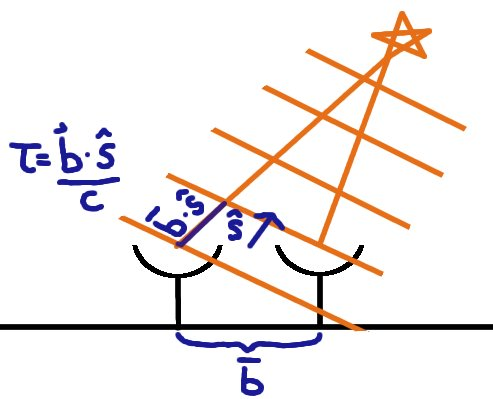
\includegraphics[width = .5\textwidth]{geometric_delay.png}
\caption{Two-interferometer system showing the derivation of the
  geometric delay. Meticulous art by Aaron Parsons, PhD.}
\end{figure}
\subsubsection{Correlation Theorem and the Architecture of Data Synthesis}
Correlation is a mathematical tool for determining the 'similarity'
level of data, or in a specific case, how alike are different signals
over a time period. The correlation of two functions is the integral of
the fourier transform of one function times the conjugated fourier
transform of the other function:
\begin{align}(f\star{g})(\tau) =
  \int{\hat{f}(\omega)\hat{g}^{\ast}(\omega)e^{i\omega{t}} d\omega}
\end{align}
For interferometry, we take g(t) to be f(t-$\tau$), where $\tau$ is the
geometric delay, to correlate data received by one radio telescope with
a delayed but similar signal received by another telescope. The
correlation relation can thus be written as:
\begin{align}f(t)\star{f(t-\tau)} =
  \int{\hat{f}(\omega)\frac{1}{2\pi}\hat{f}^{\ast}(\omega)e^{i\omega{t-\tau}}
    d\omega}
\end{align}
\begin{align}=\left|{f}^{2}\right|\int{\frac{1}{2\pi}e^{i\omega{t-\tau}}d\omega} 
  =\left|{f}^{2}\right|\cdot\delta(t-\tau)
\end{align}
It turns out that when two similar signals separated by a time delay get
correlated, the result is a delta function. The measurement as power as
function of time has peaks at the delay (positive and negative $\tau$);
correlation can be used to determine and geometric delay and thus, as we
shall see, the precise length of the baseline. In radio astronomy, data
is often preferred in frequency domain and is the case for the output of
a correlator. This process becomes cumbersome when dealing with large 
amounts of data from a large array of telescopes, but programs are
designed to lighten the load. There are two types of correlators: FX and 
XF architectures. in the XF design, the signals are correlated first and
then fourier transformed. This can take heavy amounts of processing
because, for an array of N telescopes, there are $\frac{N}{2}(N+1)$
correlations and thus such number of fourier transformations to
computer. In the more common and efficient FX architecture, the fourier
transforms are computer first, so that there are only N computations,
and then the correlations take place. FPGAs are the primary tools for
the computations with GPUs occasionally assist in the correlation.
\subsubsection{There's a Correlation! Duo-Signal Interferometry}
We now have two sets of data each with its own geometric delay
$\tau_{1}$ or $\tau_{2}$. We correlate the corresponding signals as
functions f and g with $f(t) = f_{1}(t) + f_{2}(t)$ and $g = f(t-\tau) =
f_{1}(t-\tau_{1}) + f_{2}(t-\tau_{2})$:
\begin{align}f\star{g}(\tau) = \int{f(t)f^{\ast}(t-\tau)dt} 
\end{align}
\begin{align}=
  \int{f_{1}(t)f_{1}(t-\tau_{1}-\tau)f_{2}(t)f_{2}(t-\tau_{2}-\tau)dt}
\end{align}
\begin{align}= \int{f_{1}(t)f_{1}(t)dt} = <e_{1}^{2}>
\end{align}
Equation 7 is the correlation equation. Equation 8 is obtained by
multiplying out the terms in the integrand and eliminating the product 
terms of $f_{1}(t) and f_{2}(t)$, which are integrated to 0. We then set 
$\tau = -\tau_{1}$ or $-\tau_{2}$ to get either a factor of $f_{1}^{2}$
or $f_{2}^{2}$ with the other one integrated to 0. The result in
equation 9 is an amplitude at $-\tau_{1}$ or $-\tau_{2}$, as expected
from the delta function result from the correlation theorem. There will 
be noise generated from other sources from the sky.
\begin{figure}[!h]
\centering
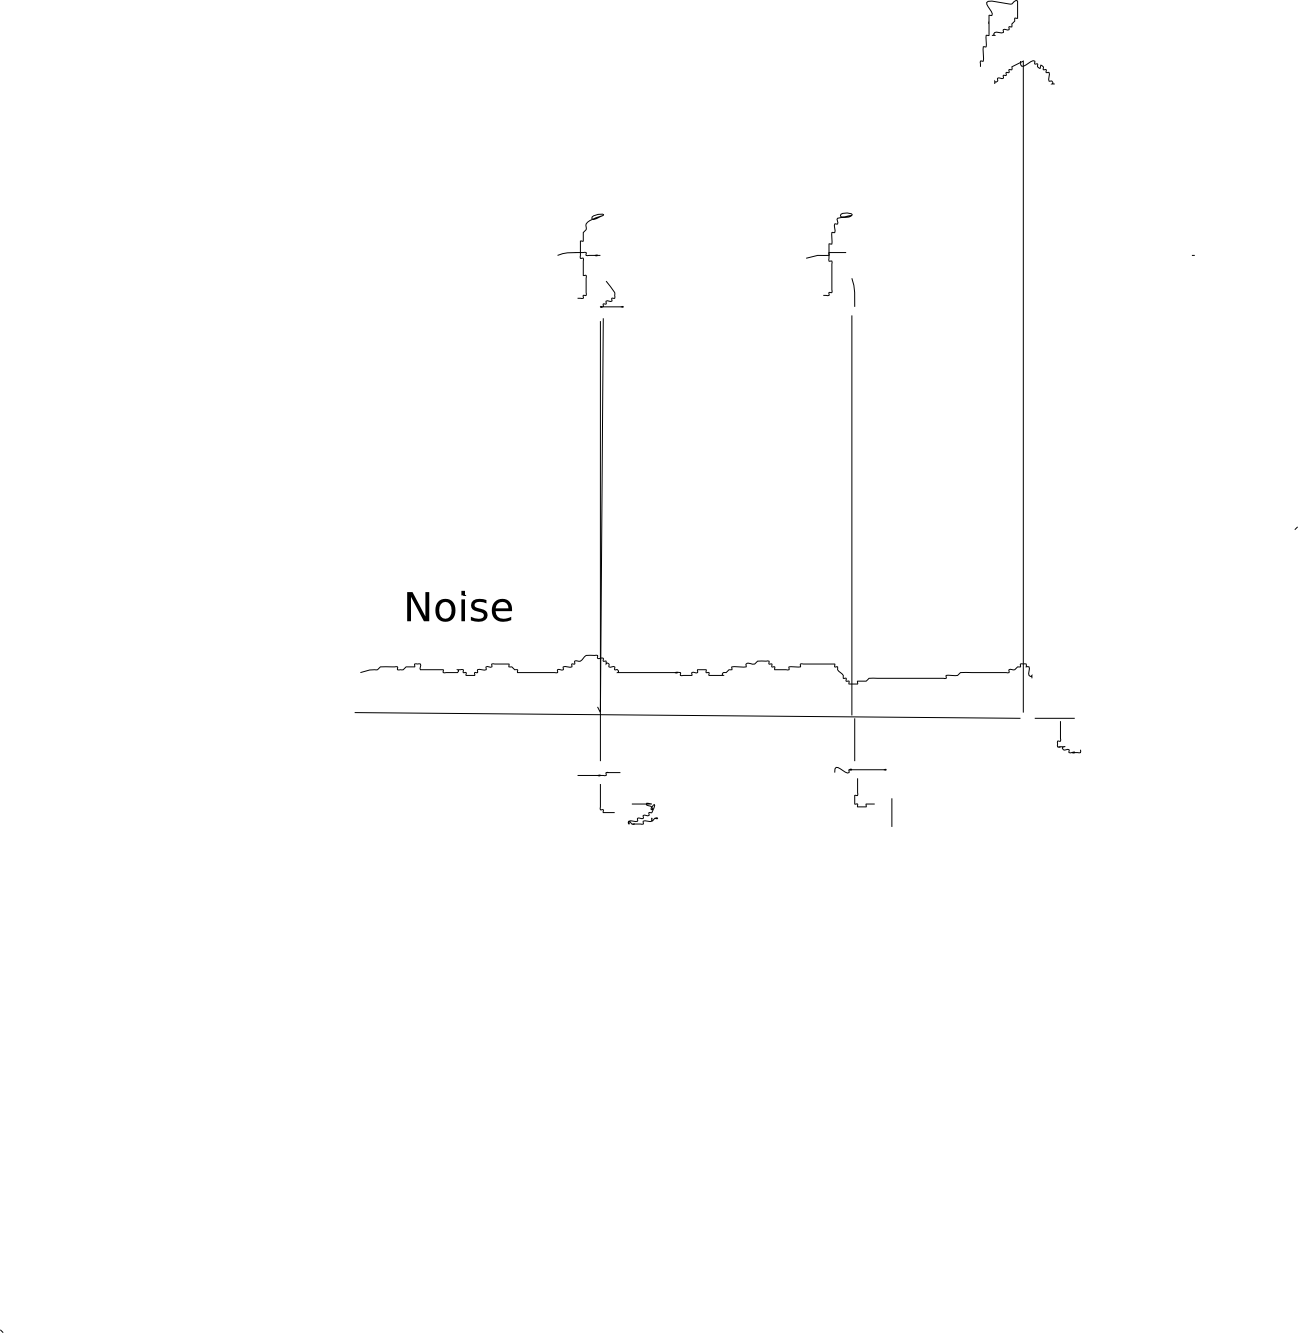
\includegraphics[width=.55\textwidth]{delay.png}
\caption{Simplified graphical representation of the correlated data with peaks at
  the corresponding delays}
\end{figure}
Two telescopes can provide only 1-D images since the geometric delay
accounts for only 1 direction; larger arrays can provide 2-D images,
reflecting what is seen in the sky.
\subsubsection{Dirtying the Sky; The Visibility Equation}
It's useful to first limit ourselves to a single frequency $\nu$ since
our analyses are often frequency dependent. We write the geometry delay
in terms of $\nu$:
\begin{align}\tau\nu =
  \frac{\overrightarrow{\textbf{b}}\cdot\hat{\textbf{s}}}{\lambda}
\end{align}
This delay gives rise to a phase difference denoted by:
\begin{align}\Delta\phi = e^{-i\theta} =
  e^{2\pi{i}\frac{\overrightarrow{\textbf{b}}\cdot\hat{\textbf{s}}}{\lambda}}
\end{align}
This complex factor in term produces a somewhat sinusoidal fringe
pattern while the real component produces a image of the sky with the
source, both as a function of distance along the sky. With this
information, it is possible to map the sky with one baseline,
representing what a larger array can image. We split the baseline into
its three components of east-west, north-south, and depth
$\frac{\overrightarrow{\textbf{b}}}{\lambda} = (u,v,w)$. Similarly, we
separate the directional unit vector $\hat{\textbf{s}}$ into east-west,
north-south, and unit factor components $(l,m,\sqrt{1-l^{2}-m^{2}}$. By
integrating the intensity I(l,m) with the response of the primary
antenna beams A(l,m) and the phase shift, we get the visibility, or
measurement, of the sky: 
\begin{align}V(u,v) = \int\int{A(l,m)\cdot{I(l,m)}\cdot
    {e^{-2\pi{i}\frac{\overrightarrow{\textbf{b}}\cdot\hat{\textbf{s}}}{\lambda}}}dldm}
\end{align}
\begin{align}= \int\int{A(l,m)\cdot{I(l,m)}\cdot
    {e^{-2\pi{i}(ul+vm+w\sqrt{1-l^{2}-m^{2}})}}}
\end{align}
\begin{align}\approx e^{-2\pi{i}w}\int\int{A(l,m)\cdot{I(l,m)}\cdot
    {e^{-2\pi{i}(ul+vm)}}}
\end{align}
Assuming l and m to be much smaller than 1, a valid assumption, the
integral simplifies down to Equation 14. The visibility equation is the
fourier transformation of the sky from spatial (angular) domain to
wavelength (inverse angular) domain, whose corresponding image is the
$'u-v plane'$. Data from a pair of telescopes come
in two samples: values for positive and negative u and v; that is, there
are measurements of V and $V^{\ast}$. Taking different values for
baseline and computing the visibility produces the sampling pattern of
the sky and its corresponding $'real'$ image of the sky known as the
$'dirty beam'$. The sampling pattern samples the true u-v plane,
resulting in a $'dirty'$ image of the sky, where the dirtying refers to
a messy image due to information loss from the sampling. 
\begin{figure}[!h]
\centering
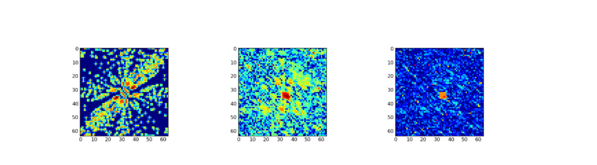
\includegraphics[width=\textwidth]{visibility.png}
\caption{Example of the visibility imaging process, courtesy of radio
  astronomer Aaron Parsons, PhD. Left: the sampling
  pattern; middle: the dirtied image; right: the cleaned image}
\end{figure}
The image can be cleaned by
deconvolution, a method that involves providing prior-known information
of the real sky to improve the smoothness of the resulting image.
\subsubsection{Resolution and the Limits of Observation}
Resolution is limited by the nature of light. The diffraction limit
under perfect observing conditions is the observed angle about which an
image can be resolved and the angle is related to light and your
instrument by: 
\begin{align}\theta \approx 1.22\frac{\lambda}{D}
\end{align}
$\lambda$ is the wavelength of the signals received and D is the
diameter of the telescope. Radio astronomical observations are minimally
affected by confounding factors in the atmosphere at appropriate
location so this diffraction limit holds true. The long wavelength of 
radio waves makes it somewhat difficult to resolve very distant sources,
but this problem is alleviated by using an array of dishes with large
values, B of the baseline that replace D.
\subsection{Least-Squares Fitting and Determining the Baseline}
The fringe data provides us with much information, including the precise
baseline of our interferometer or the precise declination of our point
source. Only one component of our baseline matters since we're working
with a two-telescope array and we denote this baseline component by
$B_{y}$. The delay of signal reception is actually more than just the
geometric delay due to electronics in the cable: $\tau_{total} =
\tau_{geo}(h_{s}) + \tau_{cable}$ where $h_{s}$ is the hour angle of the
point source. $\tau_{geo}$ can be written as a function of $B_{y}$,
declination $\delta$, and $h_{s}$:
\begin{align}\tau_{g}(h_{s}) = \frac{B_{y}}{c}cos(\delta)sin(h_{s})
\end{align}
From this, we get the total fringe voltage:
\begin{align}F(t) = E_{1}(t)\cdot E_{2}(t) = cos(2\pi\nu{t})\cdot
  cos(2\pi\nu[t+\tau_{total}])
\end{align}
Using trigonometric manipulating and changing the frequency $\nu$
dependence to wavelength $\lambda$ dependence, we arrive at the Fringe
Amplitude Equation that describes our data:
\begin{align}F(h_{s}) =
  Acos[2\pi(\frac{B_{y}}{\lambda}cos(\delta))sin(h_{s})] -
  Bsin[2\pi(\frac{B_{y}}{\lambda}cos(\delta))sin(h_{s})] 
\end{align}  
The coefficients are defined as A $\equiv
cos(\frac{2c\pi\tau_{cable}}{\lambda})$ and B $\equiv 
cos(\frac{2c\pi\tau_{cable}}{\lambda})$. This equation is now ripe to be
used with least-squares fitting on point source data. Least-squares
fitting is a method of fitting a data set to a type of curve that best
represents the data set. Our goal is to determine either the baseline or
the declination, but not both because you have to assume one to solve
for ther other as a variable. For convenience we define C $\equiv
[2\pi(\frac{B_{y}}{\lambda}cos(\delta))]$, reducing the equation to:
\begin{align}F(h_{s}) = Acos[Csin(h_{s})] - Bsin[Csin(h_{s})] 
\end{align} 
The hour angle $h_{s}$ can be obtained using your local sidereal time
and the right ascension of the source. Our least-squares method
ultimately outputs values of the residuals of our data. We plot the
values of the residuals against C and the C value corresponding to the
lowest residual value can be used to solve either $\delta$ or or $B_{y}$
by assuming one.  
\subsection{The Size of Round Stuff in the Sky}
A core goal of the interferometer is to project waves corresponding to
received data onto constructed images of the sky to represent the
information in the signals. Over time, the movement of objects across
its projected fringe pattern produces a fringe response from our
interferometer. For point sources, the fringe response F(h) is well
described by the Equation 20. For objects large enough to be
distinguishable in the sky and thus cannot be desribed by a singular
value of hour angle, their hour angle is a function is related to
intensity distribution over the sky. We use this information and the
fact that intensity as a function of hour angle is related to the source
radius to derive the size of the sources. 
\subsubsection{Mapping Round Stuff in the Sky: Brightness Distribution}
The hour angle of a sizable non-point source and the intensity
disribution of the source is given by:
\begin{align}h_{s} = \frac{\int I(h) h dh}{\int I(h) dh}
\end{align}
This equation describes the hour angle of the source center as the mean
of its intensity. We write the intensity of a non-center point of the
source as  $I(\Delta h)$ where $\Delta h$ is the difference of the hour
angle between the non-center point and the center point $h-h_{s}$. To
find the response $R(h)$ of such an 'extended' source in the sky, we
multiply Equation 20 by intensity as a function of hour angle difference
and integrate the equation over small changes in hour angle $d\delta h$:
\begin{align}F(h_{s}) =
  A\int{I(\Delta
    h)cos[2\pi(\frac{B_{y}}{\lambda}cos(\delta))sin(h_{s})] d\Delta h} +
  B\int{I(\Delta h)sin[2\pi(\frac{B_{y}}{\lambda}cos(\delta))sin(h_{s})]
  d\Delta h} 
\end{align}
To simplify numerically and conceptually, we define the local fringe
frequency $f_{f} = \frac{C}{2/pi}cos(\delta)$ where $C \equiv
\frac{B_{y}}{\lambda}cos(\delta)$. Since the Sun and Moon
have declinations near 0 around at the time of our observations,, we can
simplify the equation with the approximation $C \approx
\frac{B_{y}}{\lambda}$. Using trigonometric identities and this
definition, we come to: 
\begin{align}R(h) = F(h) \cdot \int{I(\Delta h)cos(2\pi f_{f}\Delta h)
    d\Delta h}
\end{align}
Here, F(h) refers to the source center, corresponding to a $\Delta$ h
value of 0. The integral part of the equation is the theoretical
modulation function, the intensity distribution of the source across the
sky in 1-D fourier space. The result of this equation, the brightness
distribution, as fringe response as a function of anglular difference
between source point and source center in the sky, appears symmetrically
as an inverse parabola leveling off to constant value on either side. In
fourier space, the result appears as a sinc function
$\frac{sin(2\pi{f_{f}}R)}{2\pi{f_{f}}R}$ and the inverse domain can be
in units of source diameter per fringe period. Analysis in this domain
can lead to obtaining the radius of the source.
\subsubsection{Discovering the Size: Theoretical Modulation}
$I(\Delta h)$ is convenient for us because it can be function of the source radius, which
is what we would like to know:
\begin{align}I(\Delta h) = \frac{\sqrt(R^{2}-\Delta h^{2})}{R}
\end{align}
where R is the radius of the point source. We then write the theoretical
modulating function $MF_{theory}$ in terms of R as well:
\begin{align}MF_{theory} = \frac{1}{R}\int{\sqrt(R^{2}-\Delta h^{2})cos(2\pi
    f_{f}\Delta h) d\Delta h}
\end{align} 
We want to solve for source sizes numerically, so we divide the source
intensity into 2N + 1 sections where the odd number chosen is for
symmetry about the source center. Each division has a corresponding size
and hour angle coverage of $\frac{R}{N} = \delta h$. The nth section
thus spans an hour angle of $\Delta h_{n} = n\delta h$. The numerical
form of the theoretical analytical modulating function is:
\begin{align}MF_{theorey} \approx \sum\limits_{n=-N}^{+N} \sqrt(R^{2} -
  (n\delta h)^{2})cos(2\pi{f_{f}}n\delta h) \delta h
\end{align}
\begin{align}\approx \delta
  h\sum\limits_{n=-N}^{+N}\sqrt(1-(\frac{n}{N})^{2})cos(\frac{2\pi
    f_{f}Rn}{N})  
\end{align}
The summation equation is what is important to us. For large objects
with a fringe phase offset, we first have to find the offset by using
the least-squared method akin to what is done to determine the
baseline. We then use the appropriate value for our numerical response
equation. for The parameters at play here is are the fringe amplitude,
source radius, and the local fringe frequency. There are certain values
of R and $f_{f}$, related by $\frac{1}{f_{s}} = \frac{n}{2R}$, that
correspond to 0 value for the amplitude. Once we have the these values
of $f_{s}$, we can solve for the radius of our sources, the Sun and the
Moon.  
\section{Data}
Data is collected for three sources: the Sun, the Moon, and a distant
point source, the Orion Nebula in our case. We track each source with
the two-telescope interferometer approximately from its time of rise to
its time of setting. We instruct the telescopes to track by providing to
them our latitude $(+37.8732^{\circ})$ and longitude
$(-122.2573^{\circ})$. The location to begin the observation is
determined by the location of the source that that moment, which can be
determined by its topocentric coordinates. For every observation, the
direction of the telescope returns home every hour before continuing the
data collection to prevent runaway tracking; there is a small gap once
every 3600 seconds as shown in the plots. The initial data plots had
their data points subtract out an average over a range to appear more
clean and symmetric about the x-axis. It's sometimes useful to fourier
filter the data to remove the outlier from having a significant amount
of influence in analyses, but for our purposes the difference is
negligible. 
\subsection{Solar Power}
Data for the Sun, obtained over a span of about ten hours.
\begin{figure}[H]
\centering
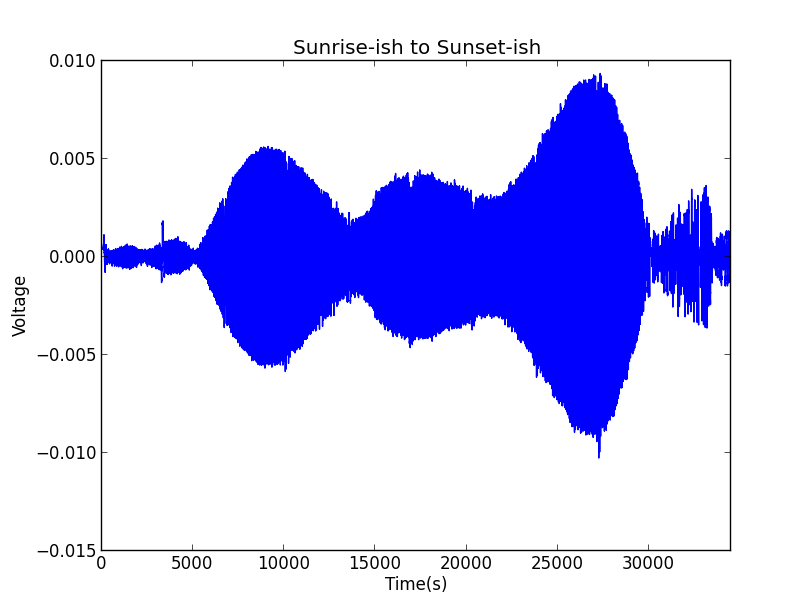
\includegraphics[width=.9\textwidth]{sun.png}
\caption{The fringe pattern of the sun from about sunrise to sunset}
\end{figure}
The Sun's data shape arises from its unique characteristics relative to
us. Its rather large occupancy of solid angles in the sky and its
sunspots influence the data we receive from it.
\subsection{Lunar Radiance}
Data for the Moon, obtained over nearly half a day.
\begin{figure}[H]
\centering
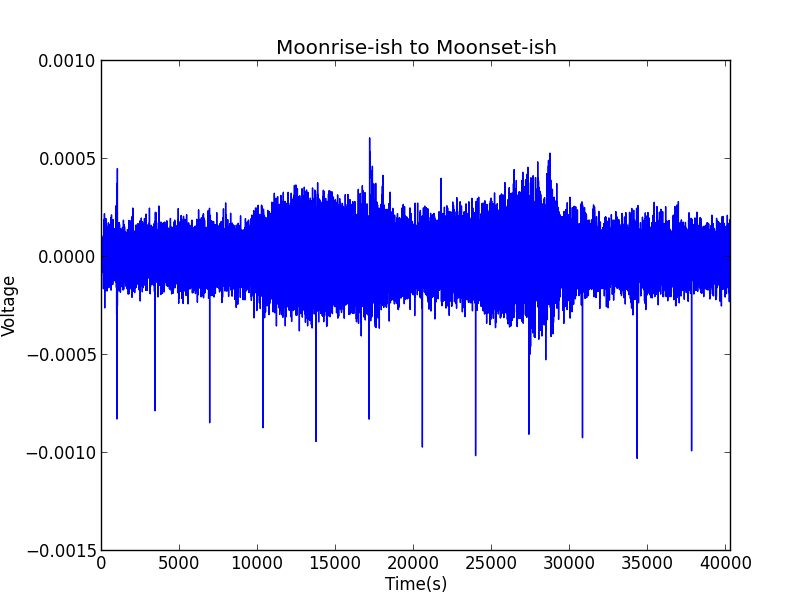
\includegraphics[width=.9\textwidth]{moon.png}
\caption{The fringe pattern of the moon from about moonrise to moonset}
\end{figure}
The Moon has a somewhat similar pattern to the Sun's but to less
extremes. It is also very big in the sky.
\subsection{Nebular Message}
Data for the Orion Nebula:
\begin{figure}[H]
\centering
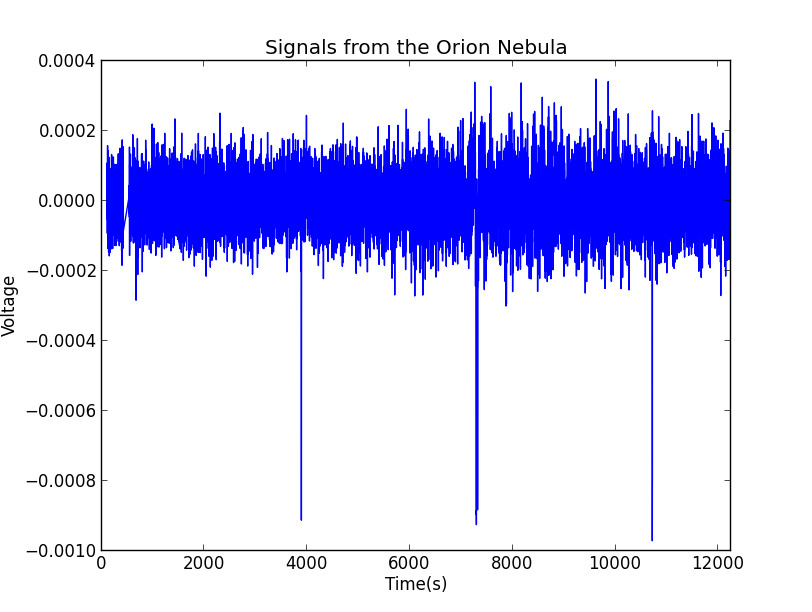
\includegraphics[width=.9\textwidth]{orion.png}
\caption{The fringe pattern of the nebula obtained over several hours}
\end{figure}
This graph is typical of that of a point source. It behaves more like a
normal sinusoid than the Sun and Moon data.
\section{Analysis and Discussion}
We apply the methods described previously to our data. We use 
least-squares fitting and the mathematical equations to derive real-time 
characteristics of the Sun, Moon, and Orion Nebula from their data.  
\subsection{Interferometer Baseline Length Extraction from Orion Data}
Recalling that C $\equiv [2\pi(\frac{B_{y}}{\lambda}cos(\delta))]$ with
$\lambda = .028$ meter from the center frequency (10.67 GHz) our
instrument operates on, we take $\delta$ to be the measured declination
of the Orion Nebula in year 2000 (negligible difference to its present
day value) to guess the correct value of for the baseline length of our
interferometer. We know also that the baseline length is approximately
10 so we take values from 9.5 to 10.5 at increments of .001 as our
guesses. We use the corresponding C values in our least-squares program
to find an accurate value of the baseline, which is determined by the
value of C that returns the smallest value of the residual of our
data. The following is the graphical representation of the resulting
residual against C values. 
\begin{figure}[H]
\centering
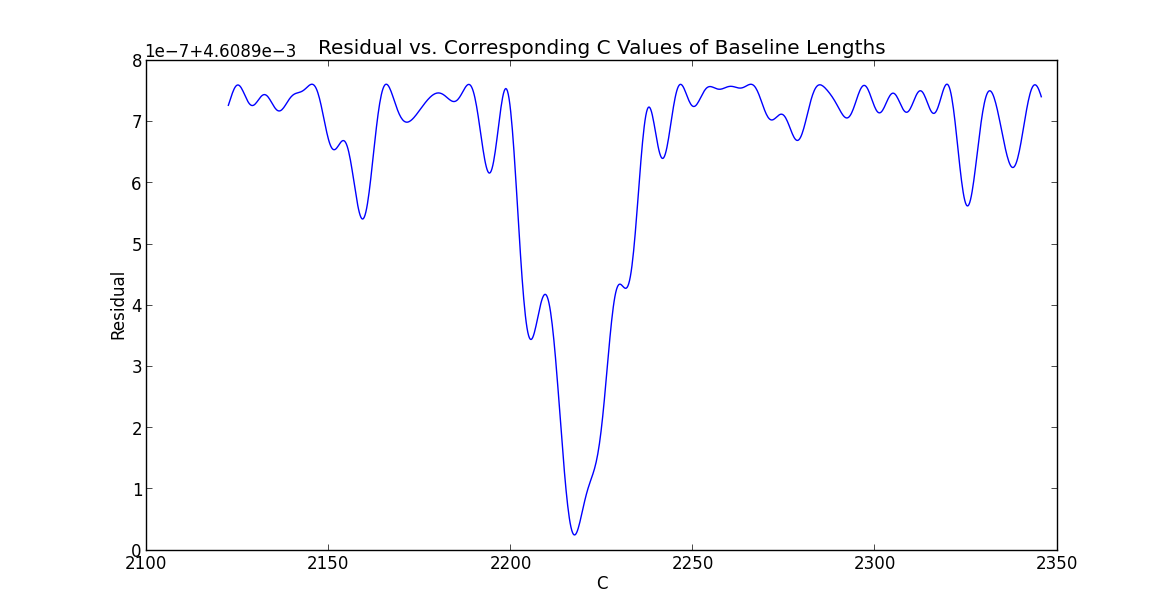
\includegraphics[width=\textwidth]{baseline.png}
\caption{A plot of the residuals of the amplitudes of our Orion Nebula
  data against guessed values of C}
\end{figure}
The value of C corresponding to the smallest value of Residual is
2217.3145. Still assuming the aforementioned value for the declination,
we arrive at the precise baseline value of \textbf{9.925 meters} for our
interferometer. Again, it's also meaningful to apply this process to
determine the declination of an object; we often can design our
interferometer knowing its precise baseline length, which knowledge is
used to pinpoint the location of objects in the sky and to determine the
limits of our resolution.
\subsection{The Waistlines of Sol and Luna}
We find the radius of the Sun and the Moon using the fringe response
equation. We are concerned with reproducing a real image so we use the
cosine component:
\begin{align}F(h) = cos(C \cdot sin(h_{S}) \cdot \phi
\end{align}
Here C is defined as usual and $\phi$ is the phase offset of our fringe
source. As aforementioned, for solar and lunar analyses, we assume
$cos(\delta)$ so be approximately 1 due to the proximity of the sources'
declinations to the celestial equator at the time of observation (near
spring equinox). C reduces to $\approx 2\pi \frac{B_{y}}{\lambda}$. We
use the baseline length we found: C $\approx 2494$. Using the
least-squares method, we find the value of $\phi$ for the Sun and the
Moon. 
\begin{figure}[H]
\centering
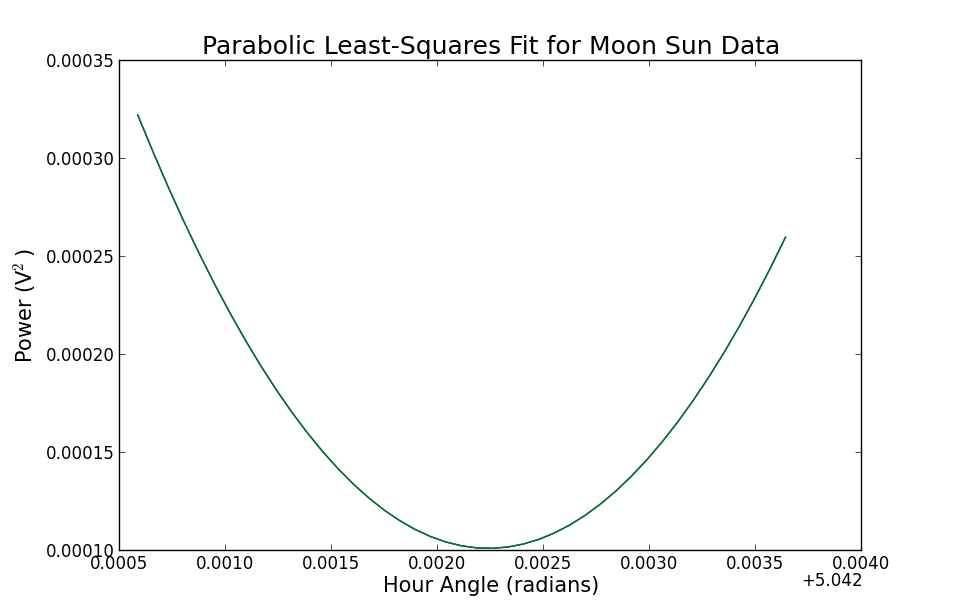
\includegraphics[width=\textwidth]{sun_fit.png}
\caption{Least-squares fit for determining $\phi$ for the sun}
The lowest value of the power corresponds to $\phi = 5.04428$ radians
for the Sun. 
\end{figure}\begin{figure}[H]
\centering
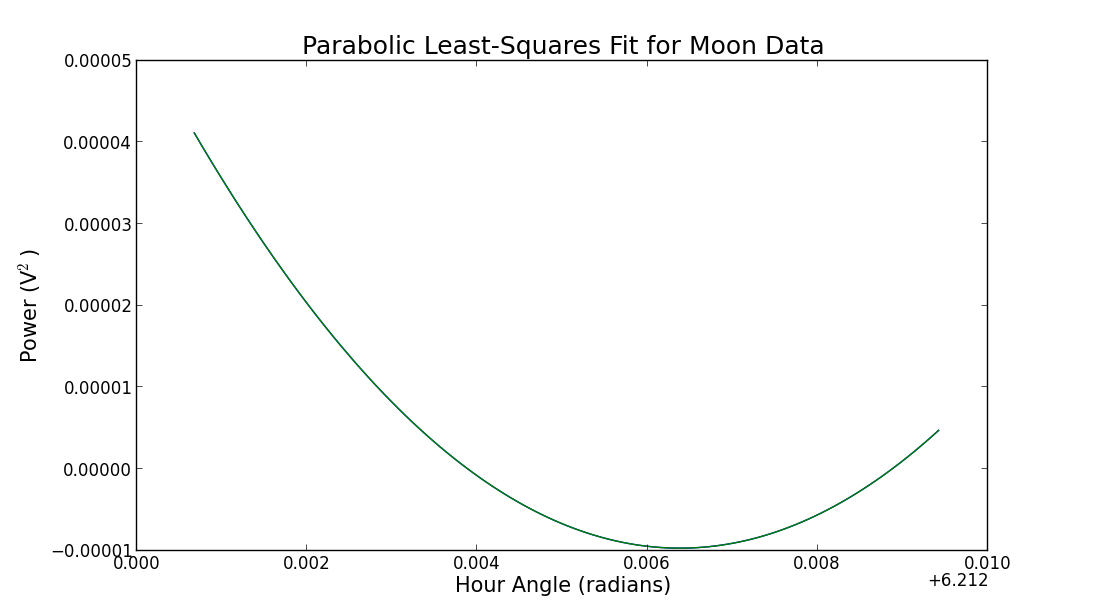
\includegraphics[width=\textwidth]{moon_fit.png}
\caption{Least-squares fit for determining $\phi$ for the moon}
\end{figure}
The lowest value of the power corresponds to $\phi = 6.21836$ radians
for the Moon. We use these $\phi$ values to solve for in our program the
Bessel polynomial function corresponding to our numerical theoretical
modulating function. We plot the resulting modulating function as a
function of $Rf_{f}$. 
\begin{figure}[H]
\centering
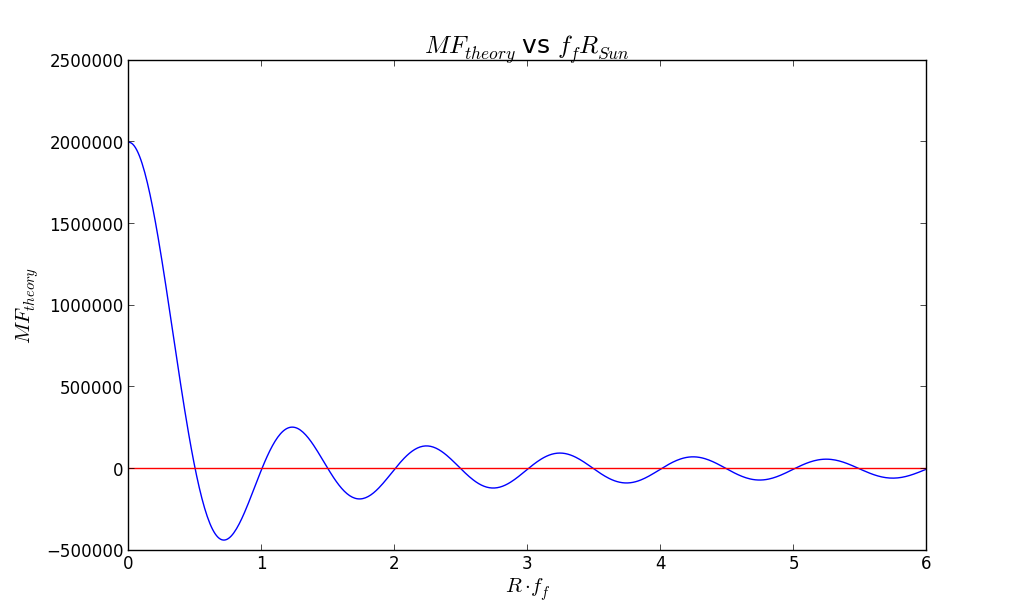
\includegraphics[width=\textwidth]{sun_MF.png}
\caption{Theoretical Modulating Function for the Moon as a function of
  $R_{Sun}$ and $f_{f,Sun}$}
There are many values of $f_{f,Sun}$ at which $MF_{theory} = 0$. We
chose $f_{s} = 115.78667$, corresponding to a radius of $R_{Sun} \approx
.00432$ radian. The Sun's radius takes up .0042 radian of the 1-D sky. 
\end{figure}\begin{figure}[H]
\centering
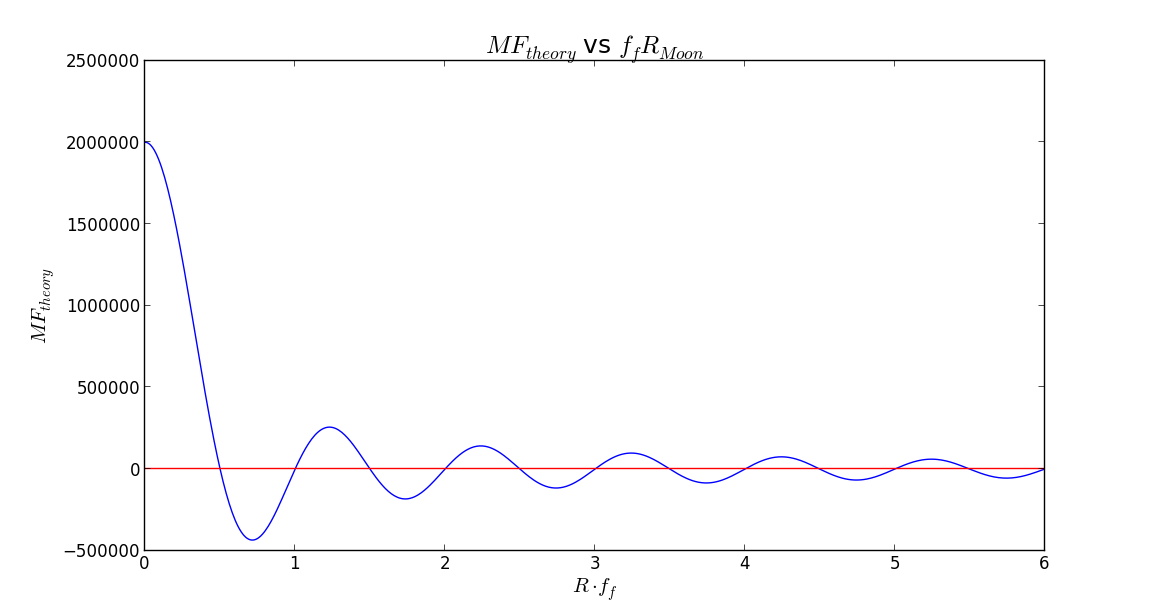
\includegraphics[width=\textwidth]{moon_MF.png}
\caption{Theoretical Modulating Function for the Moon as a function of
  $R_{Moon}$ and $f_{f,Moon}$}
Similarly, we chose 356.3204 for $f_{f,Moon}$. The corresponding radius
is $R_{Moon} \approx .0042$. Interestingly, the Sun and the Moon takes
up the same amount of angles in the sky. By sheer coincidence, their
proportional size to distance to Earth ratio, which is primarily
responsible for the results of this analysis, causes near-perfect solar
eclipses, a rare occurence elsewhere in the solar system.
\end{figure}
\section{Conclusion}
The signal from celestial sources tell us much about their
characteristics. Using interferometry, we construct fringe patterns
based on phase differences among the received signals. We ultimately can 
derive results such as a reconstructed image of the source in the sky
and characteristics such as the radius and declination of the
source. Interferometry allows us to gather and analyze information sent
by celestial objects to derive their intrisic qualities and even
information such as the precise separation of interferometer array
elements.  
\end{document}